\documentclass{sbc2023}%

\usepackage{graphicx}
%\usepackage[utf8]{inputenc}
\usepackage[misc,geometry]{ifsym} 
\usepackage{fontspec}
\usepackage{fontawesome}
\usepackage{academicons}
\usepackage{color}
\usepackage{hyperref} 
\usepackage{aas_macros}
\usepackage[bottom]{footmisc}
\usepackage{supertabular}
\usepackage{afterpage}
\usepackage{url}
\usepackage{pifont}
\usepackage{multicol}
\usepackage{multirow}
\usepackage{booktabs}
\usepackage{pgfplots}
\pgfplotsset{compat=1.16}

% Ambiente simples de pseudocódigo (flutuante), sem dependências externas
\usepackage{float}
\newfloat{algoritmo}{t}{loa}
\floatname{algoritmo}{Algoritmo}

\setcitestyle{square}

% metadados
\hypersetup{
    pdftitle={Redução Transitiva de Grafos Direcionados Baseada em Caminhamento em Profundidade},
    pdfauthor={Teixeira et al.}
}

\definecolor{orcidlogo}{rgb}{0.37,0.48,0.13}
\definecolor{unilogo}{rgb}{0.16, 0.26, 0.58}
\definecolor{maillogo}{rgb}{0.58, 0.16, 0.26}
\definecolor{darkblue}{rgb}{0.0,0.0,0.0}
\hypersetup{colorlinks,breaklinks,
            linkcolor=darkblue,urlcolor=darkblue,
            anchorcolor=darkblue,citecolor=darkblue}
%\hypersetup{colorlinks,citecolor=blue,linkcolor=blue,urlcolor=blue}

%%%%%%% IMPORTANT: We disable hyperlinks by default with this line, to avoid the error "\pdfendlink ended up in different nesting level" while writing.
%\hypersetup{draft}

\jid{JBCS}
\jtitle{Journal of the Brazilian Computer Society, 202X, XX:1, }
\doi{10.5753/jbcs.202X.XXXXXX}
\copyrightstatement{This work is licensed under a Creative Commons Attribution 4.0 International License}
\jyear{202X}


\title[Redução Transitiva de Grafos Direcionados Baseada em Caminhamento em Profundidade]{Redução Transitiva de Grafos Direcionados Baseada em Caminhamento em Profundidade}

%THE ORCID IS MANDATORY FOR EACH AUTHOR IN JBCS
\author[Teixeira et al. 2026]{
\affil{\textbf{Yrlan Rangel Teixeira}~\textcolor{blue}{\faEnvelopeO}~~[~\textbf{Pontifícia Universidade Católica de Minas Gerais}~|\href{mailto:yrlan.rangel@sga.pucminas.br}{~\textbf{\textit{yrlan.rangel@sga.pucminas.br}}}~]}

\affil{\textbf{Hugo Alves Duarte}~~[~\textbf{Pontifícia Universidade Católica de Minas Gerais}~|\href{mailto:hduarte@sga.pucminas.br}{~\textbf{\textit{hduarte@sga.pucminas.br}}}~]}

\affil{\textbf{Pedro Henrique Debs Rabelo}~~[~\textbf{Pontifícia Universidade Católica de Minas Gerais}~|\href{mailto:pedrodebs1@gmail.com}{~\textbf{\textit{pedrodebs1@gmail.com}}}~]}

\affil{\textbf{Gabriel Reis Villela}~~[~\textbf{Pontifícia Universidade Católica de Minas Gerais}~|\href{mailto:gabriel.villela@sga.pucminas.br}{~\textbf{\textit{gabriel.villela@sga.pucminas.br}}}~]}

\affil{\textbf{Gilson Júnio Pacheco Silva}~~[~\textbf{Pontifícia Universidade Católica de Minas Gerais}~|\href{mailto:gilson.pacheco@sga.pucminas.br}{~\textbf{\textit{gilson.pacheco@sga.pucminas.br}}}~]}

\affil{\textbf{Daniel Valadares Souza}~~[~\textbf{Pontifícia Universidade Católica de Minas Gerais}~|\href{mailto:danielvsouza25@gmail.com}{~\textbf{\textit{danielvsouza25@gmail.com}}}~]}

\affil{\textbf{Vinicius Figueiredo Ferreira}~~[~\textbf{Pontifícia Universidade Católica de Minas Gerais}~|\href{mailto:vinicius.ferreira.1350368@sga.pucminas.br}{~\textbf{\textit{vinicius.ferreira.1350368@sga.pucminas.br}}}~]}
}

\begin{document}

\begin{frontmatter}
\maketitle

\begin{mail}
Instituto de Ciências Exatas e Informática, Pontifícia Universidade Católica de Minas Gerais, Av. Dom José Gaspar, 500 - Coração Eucarístico, Belo Horizonte - MG, 30535-901, Brasil.
\end{mail}

\begin{dates}
% This information will be provided by the editor befeore publishing the paper
\small{\textbf{Received:} DD Month YYYY~~~$\bullet$~~~\textbf{Accepted:} DD Month YYYY~~~$\bullet$~~~\textbf{Published:} DD Month YYYY}

\end{dates}


\begin{abstract}
\textbf{Abstract.~}
\noindent A redução transitiva de um grafo direcionado $G=(V,E)$ produz um grafo $G'$ com o menor número de arestas que preserva a atingibilidade de todos os vértices de $G$. Este trabalho apresenta a implementação, em C++, de um algoritmo de redução transitiva para grafos direcionados acíclicos (DAGs) baseado em caminhamento em profundidade (DFS), com complexidade $O(|V|\cdot(|V|+|E|))$. Descrevemos a representação do grafo adotada (lista de adjacência) e a justificamos, apresentamos um verificador formal de corretude e relatamos experimentos com DAGs aleatórios de até $3{,}2\times 10^3$ vértices e $10^6$ arestas, nos quais o tempo de execução observado é compatível com a análise assintótica. Discutimos, por fim, por que o conceito de redução transitiva não se transfere diretamente para grafos não direcionados e o que ocorreria com a nossa implementação nesse cenário.
\end{abstract}

\begin{keywords}
Grafos
\end{keywords}

%\begin{license}
%Published under the Creative Commons Attribution 4.0 International Public License (CC BY 4.0)
%\end{license}

\end{frontmatter}

\section{Introdução}
\label{sec:intro}

Seja $G=(V,E)$ um grafo direcionado. A \emph{atingibilidade} de um vértice $u \in V$ é o conjunto $R_G(u)=\{v \in V \mid \text{existe caminho de } u \text{ a } v \text{ em } G\}$. Em muitas aplicações (compactação de hierarquias de dependências, visualização de grafos, fechos de ordens parciais, redes de citações) interessa o \emph{menor} subgrafo que preserva exatamente essa relação de atingibilidade. Esse subgrafo é a \emph{redução transitiva} de $G$, definida por \cite{aho1972}: um grafo $G'=(V,E')$, $E' \subseteq E$, tal que (i) $R_{G'}(u)=R_G(u)$ para todo $u \in V$ e (ii) nenhum subgrafo próprio de $G'$ satisfaz (i). Para DAGs a redução transitiva é única: uma aresta $(u,v)$ pertence a $G'$ se, e somente se, $v$ não é alcançável a partir de $u$ por nenhum caminho de comprimento maior ou igual a 2.

Este trabalho implementa a redução transitiva por meio de \emph{caminhamento no grafo}: a decisão de manter ou remover cada aresta é tomada a partir de buscas em profundidade (DFS), sem construir o fecho transitivo completo nem usar multiplicação de matrizes. A Seção~\ref{sec:impl} detalha o algoritmo e a representação adotada; a Seção~\ref{sec:exp} apresenta a metodologia experimental e os resultados; a Seção~\ref{sec:nao-dir} disserta sobre o caso não direcionado; a Seção~\ref{sec:conclusao} conclui. As responsabilidades constam da Seção~\ref{sec:resp}.

\section{Implementação}
\label{sec:impl}

O código foi organizado de forma modular, separando interfaces (\texttt{include/}) de implementações (\texttt{src/}) e dos executáveis (\texttt{apps/}): a classe \texttt{Grafo} encapsula a representação; o módulo \texttt{caminhamento} concentra as DFSs; \texttt{ReducaoTransitiva}, \texttt{Verificador} e \texttt{GeradorDag} implementam, respectivamente, o algoritmo, a verificação de corretude e a geração de instâncias; \texttt{GrafoIO} isola a E/S. Essa separação permite testar cada componente de forma independente e reutilizar o caminhamento tanto na redução quanto na verificação.

\subsection{Representação do grafo}
\label{sec:repr}

O grafo é representado por \textbf{lista de adjacência}: um vetor \texttt{adj} de $|V|$ posições em que \texttt{adj[u]} é um \texttt{std::vector<int>} com os sucessores diretos de $u$. A escolha é justificada por três fatores. Primeiro, o algoritmo é inteiramente baseado em caminhamento: uma DFS sobre lista de adjacência custa $O(|V|+|E|)$ \citep{cormen2022}, pois visita apenas as arestas que de fato existem, ao passo que sobre matriz de adjacência custaria $\Theta(|V|^2)$ por busca, mesmo em grafos esparsos; o custo total do algoritmo saltaria, assim, de $O(|V|(|V|+|E|))$ para $\Theta(|V|^3)$. Segundo, a memória é $O(|V|+|E|)$ contra $\Theta(|V|^2)$ da matriz, o que permite tratar grafos grandes e esparsos. Terceiro, a única operação que a matriz ofereceria em $O(1)$ (consultar se uma aresta específica existe) não é necessária: o algoritmo nunca pergunta ``existe $(u,v)$?'', apenas enumera sucessores. O uso de \texttt{std::vector} contíguo ainda favorece a localidade de \emph{cache} durante as travessias.

\subsection{Algoritmo de redução baseado em caminhamento}
\label{sec:alg}

A implementação explora a seguinte caracterização, válida para DAGs:

\medskip
\noindent\textbf{Propriedade.} \emph{Uma aresta $(u,v) \in E$ é transitiva (redundante) se, e somente se, existe em $G$ um caminho de $u$ até $v$ de comprimento $\geq 2$.}
\medskip

De fato, se tal caminho existe, remover $(u,v)$ não altera $R_G(u)$ (nem de nenhum outro vértice); reciprocamente, se a aresta é removível, a atingibilidade deve ser garantida por um caminho alternativo, necessariamente de comprimento $\geq 2$. Em um DAG esse caminho alternativo nunca pode usar a própria aresta $(u,v)$ ``por trás'' de um ciclo, o que torna o teste local correto.

O Algoritmo~\ref{alg:rt} aplica essa propriedade diretamente. Para cada vértice $u$, o conjunto de vértices alcançáveis por caminhos de comprimento $\geq 2$ é exatamente $\bigcup_{w \in \mathrm{adj}(u)} \bigcup_{x \in \mathrm{adj}(w)} R_G(x)$; ou seja, basta disparar DFSs a partir dos \emph{sucessores dos sucessores} de $u$, compartilhando um único vetor de marcação. Ao final, mantém-se em $G'$ somente as arestas $(u,v)$ cujo destino $v$ não foi marcado.

\begin{algoritmo}
\caption{Redução transitiva por caminhamento}
\label{alg:rt}
\hrule\vspace{1.5mm}
{\small
\textbf{Entrada:} DAG $G=(V,E)$ em lista de adjacência\\
\textbf{Saída:} redução transitiva $G'=(V,E')$\\[1mm]
\hspace*{0mm}1\ \ $E' \gets \emptyset$\\
\hspace*{0mm}2\ \ \textbf{para cada} $u \in V$ \textbf{faça}\\
\hspace*{4mm}3\ \ $\mathit{visitado}[\,\cdot\,] \gets \mathit{falso}$\\
\hspace*{4mm}4\ \ \textbf{para cada} $w \in \mathrm{adj}(u)$ \textbf{faça}\\
\hspace*{8mm}5\ \ \textbf{para cada} $x \in \mathrm{adj}(w)$ \textbf{faça}\\
\hspace*{12mm}6\ \ \textsc{DFS-Marcar}$(G, x, \mathit{visitado})$\\
\hspace*{4mm}7\ \ \textbf{para cada} $v \in \mathrm{adj}(u)$ \textbf{faça}\\
\hspace*{8mm}8\ \ \textbf{se} $\neg\mathit{visitado}[v]$ \textbf{então} $E' \gets E' \cup \{(u,v)\}$\\
\hspace*{0mm}9\ \ \textbf{devolva} $G'=(V,E')$
}
\vspace{1.5mm}\hrule
\end{algoritmo}

A rotina \textsc{DFS-Marcar} é uma busca em profundidade \emph{iterativa} (com pilha explícita), evitando estouro da pilha de execução em grafos profundos. Como o vetor \texttt{visitado} é compartilhado entre todas as DFSs disparadas para um mesmo $u$, cada vértice e cada aresta são processados no máximo uma vez por iteração externa, e o custo por vértice $u$ é $O(|V|+|E|)$. O custo total é, portanto,
\[
T(|V|,|E|) = O\!\left(|V|\cdot(|V|+|E|)\right),
\]
com espaço adicional $O(|V|)$ além do grafo. Antes da redução, o programa executa uma DFS com três cores para certificar que a entrada é acíclica, rejeitando grafos com ciclos; nesse caso a redução transitiva única não é definida sobre subconjuntos de $E$ e o tratamento adequado exigiria condensação em componentes fortemente conexas.

\subsection{Verificador de corretude}

Para sustentar a correção experimental, implementamos um verificador independente que confere as duas condições da definição: (i)~\emph{equivalência de atingibilidade}, comparando $R_G(u)$ e $R_{G'}(u)$ para todo $u$ via DFS em ambos os grafos; e (ii)~\emph{minimalidade}, certificando que nenhuma aresta remanescente de $G'$ é alcançável por caminho alternativo de comprimento $\geq 2$. O verificador foi aplicado a todos os casos de teste, incluindo instâncias clássicas (triângulo transitivo, diamante com atalho) e DAGs aleatórios de diversos tamanhos e densidades, sempre com resultado positivo.

\section{Experimentos e resultados}
\label{sec:exp}

\subsection{Metodologia}

Os DAGs de entrada foram gerados pelo modelo $G(n,p)$ ordenado: fixada uma permutação topológica implícita $1,\dots,n$, cada par $(i,j)$ com $i<j$ recebe aresta com probabilidade $p$, o que garante aciclicidade por construção. Variamos $n \in \{100, 200, 400, 800, 1600, 3200\}$ e $p \in \{0{,}01;\ 0{,}05;\ 0{,}2\}$, cobrindo regimes esparsos e densos. Os programas foram compilados com \texttt{g++ -O2} (C++17) e executados em ambiente Linux de 64 bits; os tempos referem-se exclusivamente à rotina de redução (excluindo E/S), medidos com \texttt{std::chrono}.

\subsection{Resultados}

A Tabela~\ref{tab:res} resume os resultados. Dois comportamentos merecem destaque. Primeiro, a \emph{taxa de remoção} cresce fortemente com a densidade: para $p=0{,}2$, mais de 99\% das arestas são transitivas nos grafos maiores ($n \geq 1600$), enquanto para $p=0{,}01$ e $n$ pequeno quase nada é removido, o que é coerente com a teoria, já que em DAGs densos a maioria dos pares conectados possui múltiplos caminhos. Segundo, o tempo de execução escala de forma compatível com $O(|V|\cdot(|V|+|E|))$: por exemplo, de $n=1600$ para $n=3200$ com $p=0{,}2$, $|V|$ dobra e $|E|$ quadruplica, e o tempo cresce $\approx 6{,}8\times$ (96~ms $\to$ 658~ms), próximo do fator 8 previsto pelo termo dominante $|V|\cdot|E|$.

\begin{table}[t]
\centering
\caption{Resultados da redução transitiva em DAGs aleatórios ($G(n,p)$ ordenado, semente fixa).}
\label{tab:res}
\small
\begin{tabular}{rrrrrr}
\toprule
$n$ & $p$ & $|E|$ & $|E'|$ & Remov. & Tempo (ms)\\
\midrule
100  & 0{,}01 & 47      & 47    & 0\%     & $0{,}004$\\
100  & 0{,}05 & 223     & 184   & 17\%    & $0{,}047$\\
100  & 0{,}20 & 959     & 208   & 78\%    & $0{,}095$\\
400  & 0{,}01 & 821     & 782   & 5\%     & $0{,}088$\\
400  & 0{,}05 & 3\,954  & 1\,324 & 67\%   & $1{,}16$\\
400  & 0{,}20 & 15\,814 & 882   & 94\%    & $3{,}14$\\
1600 & 0{,}01 & 12\,712 & 6\,756 & 47\%   & $12{,}4$\\
1600 & 0{,}05 & 63\,826 & 5\,715 & 91\%   & $41{,}3$\\
1600 & 0{,}20 & 255\,386 & 3\,822 & 98{,}5\% & $96{,}2$\\
3200 & 0{,}01 & 50\,938 & 15\,165 & 70\%  & $93{,}6$\\
3200 & 0{,}05 & 256\,244 & 11\,468 & 95{,}5\% & $233$\\
3200 & 0{,}20 & 1\,023\,375 & 7\,569 & 99{,}3\% & $658$\\
\bottomrule
\end{tabular}
\end{table}

\begin{figure}[t]
\centering
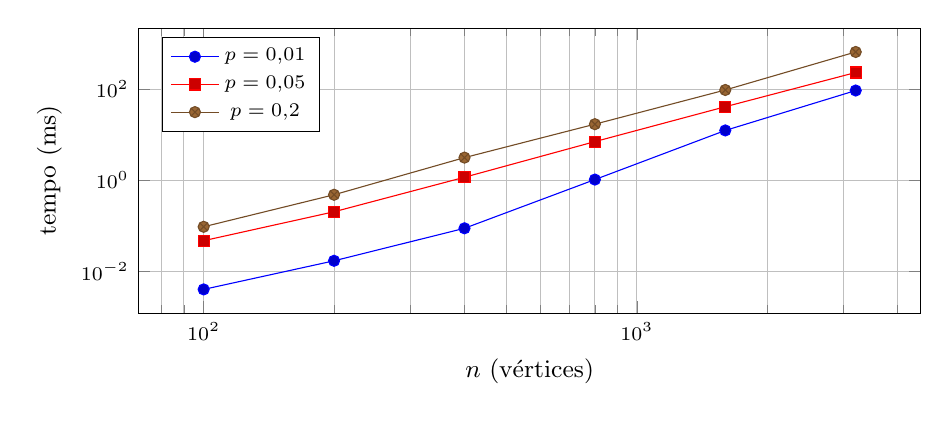
\begin{tikzpicture}
\begin{loglogaxis}[
  width=0.95\linewidth, height=5.2cm,
  xlabel={$n$ (vértices)}, ylabel={tempo (ms)},
  legend pos=north west, legend style={font=\scriptsize},
  grid=both, tick label style={font=\scriptsize},
  label style={font=\small}]
\addplot coordinates {(100,0.004) (200,0.017) (400,0.088) (800,1.035) (1600,12.425) (3200,93.634)};
\addlegendentry{$p=0{,}01$}
\addplot coordinates {(100,0.047) (200,0.203) (400,1.164) (800,7.060) (1600,41.252) (3200,233.049)};
\addlegendentry{$p=0{,}05$}
\addplot coordinates {(100,0.095) (200,0.480) (400,3.142) (800,17.059) (1600,96.210) (3200,658.214)};
\addlegendentry{$p=0{,}2$}
\end{loglogaxis}
\end{tikzpicture}
\caption{Tempo de execução em função de $n$ (escala duplamente logarítmica). A inclinação aproximadamente constante das curvas é consistente com o crescimento polinomial $O(|V|\cdot(|V|+|E|))$.}
\label{fig:tempo}
\end{figure}

A Figura~\ref{fig:tempo} apresenta o tempo em escala duplamente logarítmica. Um efeito interessante observado é que, para $p$ alto, o tempo cresce \emph{menos} que o pior caso sugere: como quase todas as arestas diretas são alcançadas logo no início das DFSs (que param em vértices já marcados), o caminhamento compartilhado por vértice efetivamente poda grande parte do trabalho.

\section{O caso não direcionado}
\label{sec:nao-dir}

A implementação \textbf{não funcionaria} para grafos não direcionados, por uma razão conceitual anterior a qualquer detalhe de código. Em um grafo não direcionado conexo, todo vértice alcança todos os demais; a atingibilidade de $u$ é simplesmente a componente conexa de $u$. O subgrafo mínimo que preserva componentes conexas é uma \emph{árvore geradora} de cada componente; ou seja, a ``redução transitiva'' de um grafo não direcionado degenera no problema de encontrar florestas geradoras, perdendo a unicidade que existe nos DAGs (qualquer árvore geradora serve, e em geral há exponencialmente muitas).

Do ponto de vista operacional, nossa implementação falharia em dois níveis. Primeiro, uma aresta não-direcionada $\{u,v\}$ corresponde ao par direcionado $(u,v)$ e $(v,u)$, formando um ciclo de comprimento 2: o teste de aciclicidade rejeitaria a entrada imediatamente. Segundo, ainda que o teste fosse suprimido, a Propriedade da Seção~\ref{sec:alg} deixa de valer: ao procurar caminhos de comprimento $\geq 2$ de $u$ a $v$, a DFS encontraria caminhos que usam a própria aresta $\{u,v\}$ no sentido inverso em outro ponto do percurso, concluindo erroneamente que a aresta é redundante. No triângulo $\{a,b\},\{b,c\},\{a,c\}$, por exemplo, \emph{toda} aresta possui caminho alternativo de comprimento 2, e o algoritmo removeria as três simultaneamente, desconectando o grafo, quando o correto (como árvore geradora) seria remover exatamente uma. A remoção precisa ser \emph{sequencial e reavaliada} no caso não direcionado (na linha do algoritmo de Kruskal/DFS para árvores geradoras), enquanto no DAG as decisões por aresta são independentes entre si, que é precisamente o que torna o caminhamento direto correto e eficiente.

O caminho correto para grafos direcionados \emph{com ciclos}, por sua vez, seria condensar as componentes fortemente conexas (Tarjan/Kosaraju), reduzir o DAG de condensação e substituir cada componente por um ciclo hamiltoniano interno mínimo, conforme observado por \cite{aho1972}.

\section{Conclusão}
\label{sec:conclusao}

Implementamos em C++ a redução transitiva de DAGs por caminhamento em profundidade, com complexidade $O(|V|\cdot(|V|+|E|))$, representação por lista de adjacência justificada pela natureza do algoritmo, e corretude atestada por um verificador independente de atingibilidade e minimalidade. Os experimentos confirmam o comportamento assintótico previsto e evidenciam que, em DAGs densos, a quase totalidade das arestas é redundante, o que reforça o valor prático da operação. Como trabalho futuro, destacam-se a extensão a grafos cíclicos via condensação de componentes fortemente conexas e a paralelização do laço externo, trivialmente paralelizável por vértice.

\section{Responsabilidades}
\label{sec:resp}

As atividades necessárias para a realização deste trabalho foram distribuídas entre os membros do grupo de acordo com a responsabilidade atribuída a cada um. A implementação do lista de adjacência foi desenvolvida por \textbf{Vinicius Figueiredo Ferreira}, o algoritmo de busca em profundidade foi responsabilidade de \textbf{Hugo Alves Duarte}, o algoritmo de redução de transitividade foi implementado por \textbf{Yrlan Rangel Teixeira}, o gerador de instâncias por \textbf{Gabriel Reis Villela}, o verificador de corretude por \textbf{Daniel Valadares Souza}, a escrita do relatório e realização dos testes e benchmark foram realizados por \textbf{Pedro Henrique Debs Rabelo} e \textbf{Gilson Júnio Pacheco Silva}.

\bibliographystyle{apalike-sol}
\bibliography{refs}

\end{document}
